\documentclass[14pt,a4paper]{report}
%\documentclass[master]{disser}
\usepackage{extsizes}% нестандартный 14-ый размер шрифта
\usepackage[left=30mm,right=15mm,top=20mm,bottom=20mm,binding offset=0cm]{geometry} % поля страницы
\usepackage[utf8]{inputenc} % Кодировка текста
\usepackage[T1,T2A]{fontenc} % Кодировка шрифта
\usepackage[english,russian]{babel} % языковая поддержка
\usepackage{indentfirst} % первый параграф раздела начинается с красной строки
\usepackage{misccorr} % исправляет некоторые несоответствия с правилами полиграфии
\usepackage{amssymb,amsmath,amsfonts,latexsym,mathtext} %расширенные наборы математических символов
\usepackage{pdfpages}
\usepackage{listings}
\usepackage{xcolor}
\usepackage{longtable}
\usepackage{lipsum}
\usepackage{biblatex}
\usepackage{filecontents}
\usepackage{enumitem}
\usepackage{hyperref}
\usepackage{caption}
\usepackage{graphicx}
\usepackage[autostyle]{csquotes}
\usepackage{amssymb}
%\usepackage{ntheorem}
\usepackage{amsthm}

\newtheoremstyle{break}
  {\topsep}{\topsep}%
  {\itshape}{}%
  {\bfseries}{}%
  {\newline}{}%

\theoremstyle{plain}

\newtheorem*{definition1}{Определение}
\newtheorem*{theorem1}{Теорема}
\newtheorem*{lemma1}{Лемма}

\newtheorem{definition}{Определение}
\newtheorem{theorem}{Теорема}
\newtheorem{lemma}{Лемма}

\theoremstyle{break}
\newtheorem*{theorem_break1}{Теорема}

\setlist[enumerate]{leftmargin=1cm,topsep=0pt,itemsep=-1ex,partopsep=1ex,parsep=1ex,ref=\arabic{*},label=\arabic{*}.}

\setlength\parindent{1cm}

\linespread{1.3} % полуторный межстрочный интервал

%Нумерация странниц
\usepackage{fancyhdr} % пакет для установки колонтитулов
\pagestyle{fancy} % смена стиля оформления страниц
\fancyhf{} % очистка текущих значений
\fancyhead[LE,RO]{}
\fancyhead[LO,RE]{}
\fancyfoot[CE,CO]{}
\fancyfoot[LE,RO]{}
\fancyhead[C]{\thepage} % установка верхнего колонтитула
\renewcommand{\headrulewidth}{0pt} % убрать разделительную линию

\frenchspacing % везде одинарные пробелы в тексте

\title{SCIENTIFIC WORK} % название документа

\addbibresource{chapters/references.bib}

\begin{document} % начало тела документа

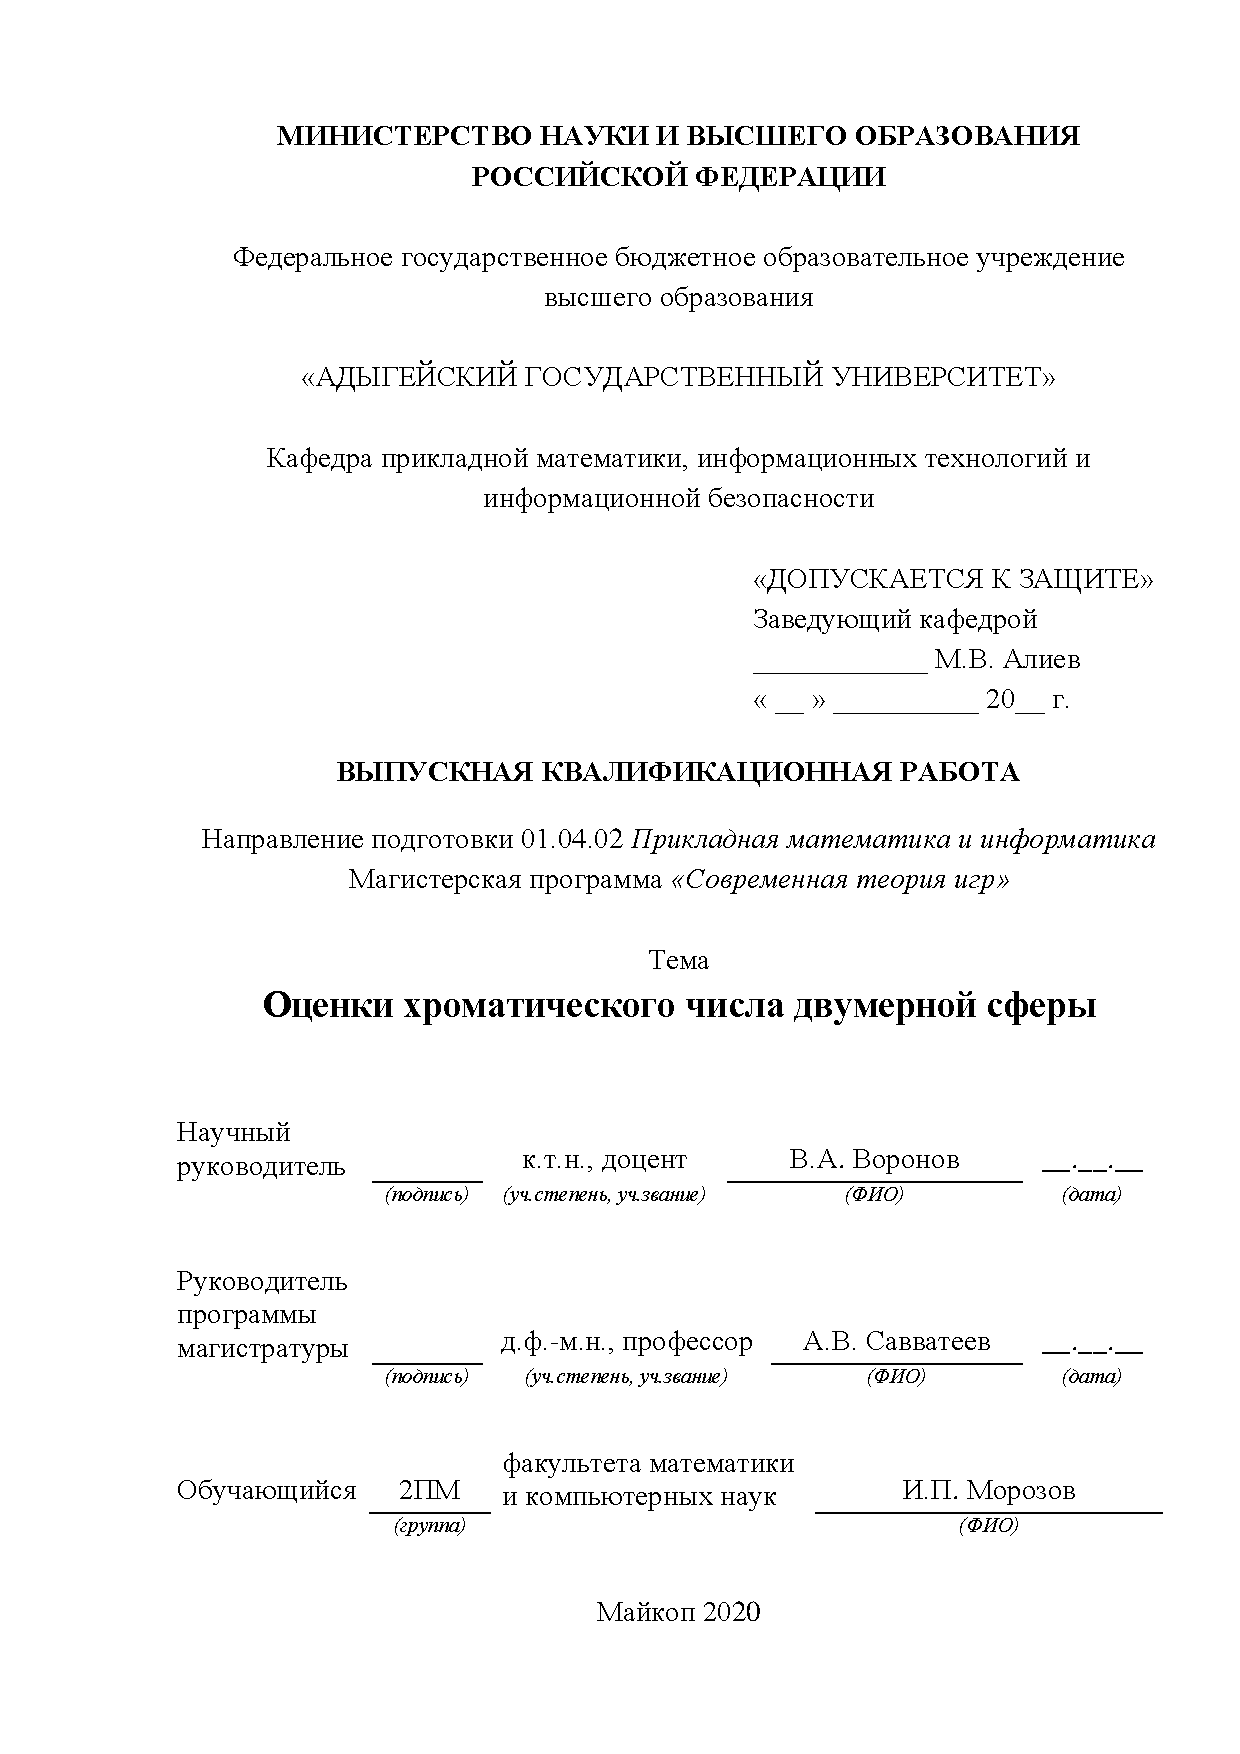
\includepdf[pages=-]{chapters/title.pdf}


\newpage

% \thispagestyle{empty} % неотображает номер страницы %

\begin{center}
\textbf{СОДЕРЖАНИЕ}
\end{center}
\vspace{1.5mm}

\begin{description}

\item{ВВЕДЕНИЕ} \dotfill \pageref{chapters:introduction}

\item{ГЛАВА 1.} РАСКРАСКИ СФЕР \dotfill \pageref{chapters:1}
\begin{enumerate}
\item[1.1] Постановка задачи и известные результаты \dotfill \pageref{chapters:1.1}
\item[1.2] Разбиение на области Вороного \dotfill \pageref{chapters:1.2}
\item[1.3] Задача Томсона \dotfill \pageref{chapters:1.3}
\end{enumerate}

\item{ГЛАВА 2.} ЗАДАЧА ВЫПОЛНИМОСТИ БУЛЕВЫХ ФОРМУЛ И SAT-РЕШАТЕЛИ \dotfill \pageref{chapters:2}
\begin{enumerate}
\item[2.1] Определения \dotfill \pageref{chapters:2.1}
\item[2.2] Алгоритм DPLL \dotfill \pageref{chapters:2.2}
\item[2.3] Алгоритм CDCL \dotfill \pageref{chapters:2.3}
\item[2.4] Детали реализации современных SAT-решателей \dotfill \pageref{chapters:2.4}
\end{enumerate}

\item{ГЛАВА 3.} ВЕРХНИЕ ОЦЕНКИ ХРОМАТИЧЕСКИХ ЧИСЕЛ СФЕР \dotfill \pageref{chapters:3}
\begin{enumerate}
\item[3.1] Численные эксперименты \dotfill \pageref{chapters:3.1}
\item[3.2] Теоретические оценки \dotfill \pageref{chapters:3.2}
\end{enumerate}

\item{ЗАКЛЮЧЕНИЕ} \dotfill \pageref{chapters:conclusions}
\item{СПИСОК ИСПОЛЬЗОВАННЫХ ИСТОЧНИКОВ} \dotfill \pageref{chapters:biblio}

\item{ПРИЛОЖЕНИЕ 1. ДИАПАЗОНЫ ЗНАЧЕНИЙ РАДИУСА ДЛЯ РЕШЕНИЙ ЗАДАЧИ ТОМСОНА} \dotfill \pageref{attachments:1}
\item{ПРИЛОЖЕНИЕ 2. КОДИРОВАНИЕ ЗАДАЧИ РАСКРАСКИ ГРАФА} \dotfill \pageref{attachments:2}
\item{ПРИЛОЖЕНИЕ 3. ВЫЧИСЛЕНИЕ ГРАНИЦ ДИАПАЗОНОВ ЗНАЧЕНИЙ РАДИУСА} \dotfill \pageref{attachments:3}
\item{ПРИЛОЖЕНИЕ 4. ПОСТРОЕНИЕ ДИАГРАММЫ ВОРОНОГО С ИКОСАЭДРАЛЬНОЙ СИММЕТРИЕЙ} \dotfill \pageref{attachments:4}
\item{ПРИЛОЖЕНИЕ 5. ВИЗУАЛИЗАЦИЯ РАСКРАСОК} \dotfill \pageref{attachments:5}

\end{description}


%\pagenumbering{arabic}

\newpage
\begin{center}
\noindent\textbf{ВВЕДЕНИЕ}\label{chapters:introduction}
\vspace{1.5mm}
\end{center}

Целью настоящей дипломной работы является получение конструктивных верхних оценок для хроматического числа двумерной сферы, 
то есть построения таких раскрасок сферы, при которых точки, находящиеся на единичном расстоянии, раскрашены по-разному. 
Это задача примыкает к области классических исследований плотнейших упаковок и редчайших покрытий сфер, находится на стыке
теории графов, комбинаторной геометрии и теории кодирования.
Актуальность данной работы обусловлена отсутствием конструктивных методов получения раскрасок сфер и слабой изученностью рассматриваемой задачи, в отличие от асимптотики хроматических чисел $n$-мерных сфер при $n\to\infty$. 
В работе рассматривается семейство раскрасок, полученных как разбиение сферы на области Вороного для решений задачи Томсона.

Для достижения поставленной цели необходимо решить следующие задачи:

\begin{enumerate}[leftmargin=1cm,topsep=0pt,itemsep=-1ex,partopsep=1ex,parsep=1ex,label=\arabic{*}.]

\item Cвести задачу о раскраске графа в $m$ цветов к задаче булевой выполнимости.
\item Провести исследование алгоритмов и методов, применяемых при построении современных \textit{SAT}-решателей.
\item Применить \textit{SAT}-решатели для поиска хроматического числа графов и получить корректные раскраски сфер, вычислить диапазоны радиусов.
\item Получить оценки хроматических чисел сфер на основе решений задачи Томсона о минимуме потенциала системы $k$ точечных зарядов на сфере и разбиений на области Вороного.
\item Доказать нижние оценки для хроматических чисел квадратов двойственных графов (триангуляций Делоне).

\end{enumerate}

Рассматриваемая задача тесно связана с классической задачей Нелсона -- Эрдёша -- Хадвигера о хроматическом числе $\chi(\mathbb{R}^2)$ континуального графа, вершинами которого являются точки плоскости, причем ребрами соединены вершины, находящиеся на единичном евклидовом расстоянии. Иными словами, требуется раскрасить плоскость в конечное число цветов так, чтобы точки, находящиеся на единичном расстоянии, имели разный цвет. Какое наименьшее число цветов для этого потребуется? В настоящее время известно, что $5 \leq \chi(\mathbb{R}^2) \leq 7$. Если вторая оценка тривиальна и основана на раскраске гексагонального замощения (\figurename{ \ref{introduction:fig:plane}}), то оценка снизу была получена Хойле [\ref{bib:Heule2018}] лишь в 2018 году при помощи компьютерных вычислений. 

\begin{figure}[h]
\centering
\captionsetup{justification=centering}
\center{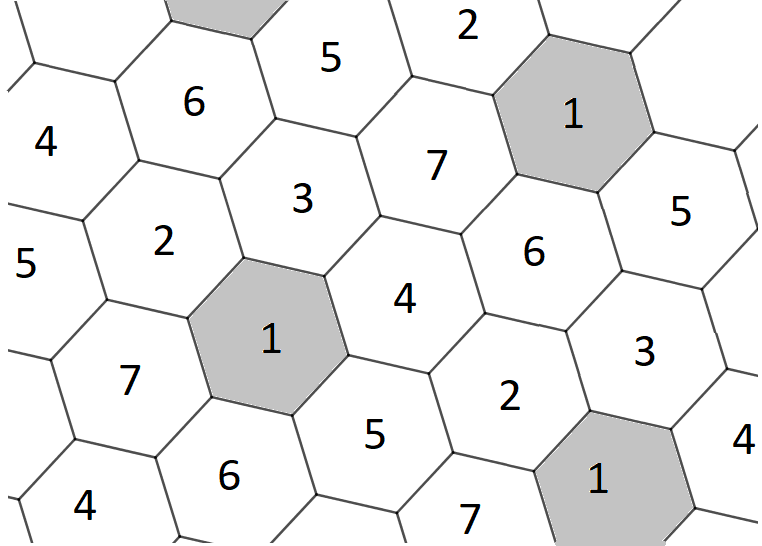
\includegraphics[width=0.4\paperwidth]{chapters/introduction/plane.png}}
\caption{Раскраска плоскости в 7 цветов.}
\label{introduction:fig:plane}
\end{figure}

Аналогичную задачу можно поставить для произвольного метрического пространства. Известно, что 
$6 \leq \chi(\mathbb{R}^3) \leq 15$ [\ref{bib:Nech}, \ref{bib:Coul}], 
получены ряд оценок для $\chi(\mathbb{R}^n)$ при $n \ge 3$, а также асимптотика $\chi(\mathbb{R}^n)$ при $n\to\infty$: 
$(1.239...+o(1))^n\leq \chi(\mathbb{R}^n)\leq (3+o(1))^n$ [\ref{bib:Rai1}, \ref{bib:Larm}].
Также рассматривались хроматические числа рациональных пространств $\mathbb{Q}^n$, многомерных сфер $S^n(r)$, 
множеств вида $\mathbb{R}^2 \times \left[ 0,~\varepsilon \right]^{k}$, ограниченных множеств, точек плоскости с координатами, принадлежащими некоторому квадратичному расширению $\mathbb{Q}$, хроматические числа пространств с запрещенными одноцветными треугольниками. Как правило, полагают, что расстояние между точками множества индуцировано евклидовой метрикой $\mathbb{R}^n$. Основополагающим результатом в данной области является следующая теорема [\ref{bib:BruijnErdos}].

\begin{theorem1}[Эрдеш -- де Брейне]
Если $G$ -- граф с множеством вершин произвольной мощности, и $\chi(G) = k$. Тогда найдется конечный подграф  $\widetilde{G} \subseteq G$, для которого $\chi(\widetilde{G}) = k$. 
\end{theorem1}

Это означает, что наилучшую из возможных оценок хроматического числа снизу всегда можно обосновать, перебирая подграфы с конечным числом вершин. Препятствием для осуществления такого перебора (даже в случае $\mathbb{R}^2$) является, во-первых, комбинаторный взрыв, а во-вторых, отсутствие методов, позволяющих раскрасить континуальный граф в тех случаях, когда критический подграф (предположительно) найден.

Отдельный класс задач возникает в том случае, если на раскраску накладываются дополнительные ограничения, например, измеримость каждого из множеств, раскрашенных в один из цветов. Еще более жесткое условие -- выпуклость компонент связности одноцветных подмножеств, 
для плоскости -- раскраска многоугольных областей. Тогда для раскраски двумерного гладкого многообразия, удовлетворяющего определенным условиям, требуется не менее 7 цветов [\ref{bib:Soifer},\ref{bib:Kronk}].


\newpage
\begin{center}
\noindent\textbf{ГЛАВА 1. РАСКРАСКИ СФЕР}\label{chapters:1}
\vspace{1.5mm}
\end{center}

\vspace{5pt}
\textbf{1.1 Постановка задачи и известные результаты}\label{chapters:1.1}
\vspace{5pt}

Графом называется пара $G=(V,~E)$, где $V$ - вершины графа, $E \subseteq \{\, (u,v) \mid u,v \in V \,\}$ - ребра графа. 
Хроматическим числом графа $\chi(G)$ называется минимальное число $k$ такое, что множество вершин $V$ можно разбить (покрасить) на $k$ 
непересекающихся классов $V_1 \sqcup V_1 \sqcup \dots \sqcup V_k = V$ так, что никакое ребро из $E$ не соединяет вершины одного класса. 
В данной работе рассматривается задача о хроматическом числе двумерной сферы 
$S^2(r) = \{\, x \in \mathbb{R}^3 : \|x\| = r \,\}$, сформулированная Полом Эрдёшем в 1981 году [\ref{bib:ErdosGraham}].
Предполагается, что расстояние между точками сферы $x,y \in S^2(r)$ задано евклидовой метрикой в $\mathbb{R}^3$: 
$d(x,y) = \sqrt{\sum_{i=1}^{3}(x_i-y_i)^2}$. Тогда 
$\chi(S^2(r)) = \min \{\, k: S^2(r) = V_1 \sqcup \dots \sqcup V_k , \, x,y \in V_i \Rightarrow \|x - y\| \ne 1 \,\}$. 
Во всех случаях, когда требуются непосредственные вычисления, предполагается, что центр сферы находится в начале координат.

Очевидно, что $\chi(S^2(r))$ зависит от $r$: если $r < \tfrac{1}{2}$, то $\chi(S^2(r))=1$, в то же время 
$S^2\left(\tfrac{1}{2}\right) = 2$ (подходит любая раскраска, в которой диаметрально противоположные точки имеют разный цвет).
При $r > \tfrac{1}{2}$ выполнено $\chi(S^2(r))>2$, так как соответствующий континуальный граф $G(S^2(r); 1)$ содержит нечетный цикл, для раскраски которого необходимы по крайней мере $3$ цвета.
В статье [\ref{bib:Simmons}] Симмонса был получен следующий результат:

\begin{theorem1}[Симмонс, 1976]
$$ \chi\left(S^2\left(\frac{1}{\sqrt{2}}\right)\right)=4, \quad \chi(S^2(r)) \geq 4 \text{ при } r > \frac{1}{\sqrt{3}}. $$
\end{theorem1}

Последнее неравенство было получено вложением в сферу конструкции, аналогичной \enquote{свернутому} веретену Мозера (\figurename{ \ref{chapter1:fig:simmons}}), для раскраски которой необходимо $4$ цвета. 
Отметим, что раскраска сферы $\chi\left(S^2\left(\frac{1}{\sqrt{2}}\right)\right)$ возникает в некой задаче квантовой механики, вследствие чего этот результат был переоткрыт другими авторами. Случай интересен тем, что $d(u,v)=1$ эквивалентно $(u,v)=0$ .
Из неравенства $\chi(\mathbb{R}^3) \leq 15$ следует, что 
$$\forall r>0 \quad \chi(S^2(r)) \leq 15.$$

\begin{figure}[h]
\centering
\captionsetup{justification=centering}
\begin{minipage}[h]{0.5\linewidth}
\center{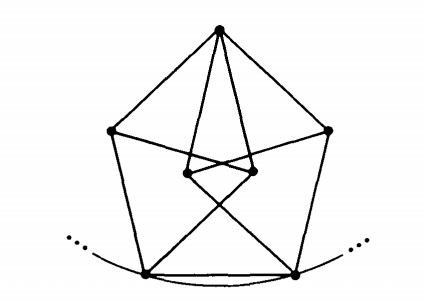
\includegraphics[width=0.4\paperwidth]{chapters/chapter1/simmons2.png}}
\end{minipage}\hfill
\begin{minipage}[h]{0.5\linewidth}
\center{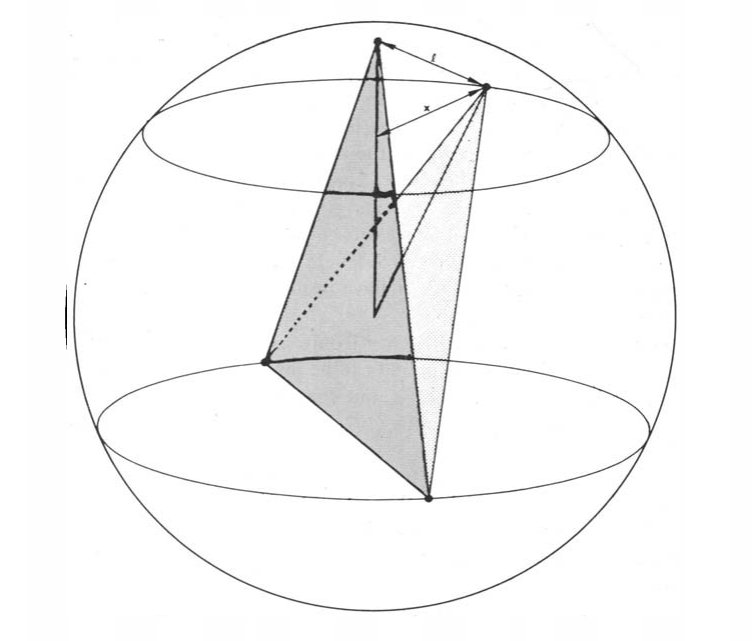
\includegraphics[width=0.4\paperwidth]{chapters/chapter1/simmons.png}}
\end{minipage}\hfill
\caption{К теореме Симмонса.}
\label{chapter1:fig:simmons}
\end{figure}

В дополнение к предыдущим рассмотрим некоторые асимптотические оценки и оценки для . В 1983 году  Л. Ловас доказал, что  $\chi(S^{n-1}(r)) \geq n$. В статье [\ref{bib:RaiSphere}] А.М. Райгородским показал, что хроматическое число сферы растет экспоненциально при росте размерности для всех $r > \frac{1}{2}$.

\begin{theorem1}

$$\text{Если } r \in (\frac{1}{2}, \frac{1}{\sqrt{2}}], \text{ то } 
\chi(S^{n-1}(r)) \geq \left(2(\frac{1}{8r^2})^{\frac{1}{8r^2}}(1-\frac{1}{8r^2})^{1-\frac{1}{8r^2}}+o(1)\right)^n.$$ 

$$\text{Если } r \geq \frac{1}{\sqrt{2}}, \text{ то } 
\chi(S^{n-1}(r)) \geq \left(2(\frac{1}{4})^{\frac{1}{4}}(\frac{3}{4})^{\frac{3}{4}}+o(1)\right)^n.$$

\end{theorem1}
В работе [\ref{bib:Kostina}] О. Костина доказала усиленный вариант предыдудщей теоремы.

\begin{theorem1}
Пусть $r > \tfrac{1}{2}$ и $b_1, b_{-1}$ таковы, что $b_1 + b_{-1} \in (0,1]$ и $b_1 < b_{-1}$.
Пусть $k_1=[b_1n]$ и $k_{-1}=[b_{-1}n]$. Положим

$$p_0(r,b_1,b_{-1},n) = \frac{(k_1 + k_{-1})n - (k_1 + k_{-1})^2}{2nr^2}$$
Пусть $p(r,b_1,b_{-1},n)$ - минимальное простое число, строго большее, чем $p_0$. 
Если при данных $r,b_1,b_{-1},n$ выполнено $k_1 + k_{-1} - 2p < -2k_{-1}$, то

$$\chi(S^{n-1}(r)) \geq 
\frac{\binom{n}{k_1}\binom{n-k_1}{k_{-1}}}
{\sum\limits_{(m_1,m_2) \in \mathcal{A}} \binom{n}{m_1} \binom{n-m_1}{m_2}}$$
где $\mathcal{A} = \{ (m_1,m_2): m_1,m_2 \in \mathbb{N} \cup \{ 0 \}, m_1+m_2 \leq n, m_1+2m_2 \leq p-1 \}$.

\end{theorem1}

Очевидно, что $\chi(S^{n-1}(r)) \leq \chi(\mathbb{R}^n) \leq (3+o(1))^n$, т.к. $S^{n-1}(r)$ лежит в $\mathbb{R}^n$. В общем случае лучших верхних оценок нет. Однако К.А. Роджерс [\ref{bib:Rogers}] получил более точную оценку в случае $r < \frac{3}{2}$.

\begin{theorem1}
$$\text{Если } r < \frac{3}{2}, \text{ то } \chi(S^{n-1}(r)) \leq (2r+o(1))^n.$$
\end{theorem1}

В работе [\ref{bib:Pros}] Р. Просановым получена следующая верхняя оценка хроматического числа сферы:

\begin{theorem1}
$\chi(S_r^{n-1}) \leq (x(r)+o(1))^n$, где
$$ x(r) = 
\begin{cases}
\sqrt{5-\frac{2}{r}+4\sqrt{1-\frac{5r^2-1}{4r^4}}},& \quad r > \frac{\sqrt{5}}{2} \\ 
2r,& \quad \frac{1}{2} < r \leq  \frac{\sqrt{5}}{2}
\end{cases}.$$
\end{theorem1}

\vspace{5pt}
\textbf{1.2 Разбиение на области Вороного}\label{chapters:1.2}
\vspace{5pt}

\vspace{5pt}
\textbf{1.3 Сферическая диаграмма Вороного}\label{chapters:1.3}
\vspace{5pt}


\newpage
\begin{center}
\noindent\textbf{ГЛАВА 2. ЗАДАЧА ВЫПОЛНИМОСТИ БУЛЕВЫХ ФОРМУЛ И SAT-РЕШАТЕЛИ}\label{chapters:2}
\vspace{1.5mm}
\end{center}

\vspace{5pt}
\textbf{2.1. Определения}\label{chapters:2.1}
\vspace{5pt}

Конъюнктивной нормальной формой (КНФ) называются булева формула вида 
$\Phi_m \left( x_1, x_2, \dots, x_m \right) = D_1 \land D_2 \land \dots \land D_k$,
где каждый дизъюнкт $D_j=t_{j,1} \lor t_{j,2} \lor \dots \lor t_{j,n_j}$, 
и все литералы $t_{j,i}$ – либо переменные, либо их отрицания,
причем переменная может встречаться в дизъюнкте не более одного раза. 
Задача выполнимости КНФ (\textit{ВЫП}, \textit{SAT}) заключается в следующем: для входной формулы $\Phi_m$ указанного вида 
необходимо определить, существует ли набор значений переменных $\left( \alpha_1, \alpha_2, \dots, \alpha_m \right)$ такой,
что $\Phi_m \left( \alpha_1, \alpha_2, \dots, \alpha_m \right) = 1$, выполнима ли $\Phi_m$? 
При этом исследователя часто интересует не только ответ \enquote{да} или \enquote{нет}, но и сам выполняющий набор переменных или доказательство его отсутствия.

Факт принадлежности задачи \textit{ВЫП} к классу $\mathcal{NP}$ является тривиальным. Более содержательное утверждение, 
знаменитая теорема Кука-Левина, открывшее важность этой задачи для теории сложности вычислений, 
а впоследствии и для практических приложений, доказал в 1971 году Стивен Кук (тот же результат независимо получило советский математик Леонид Левин). В своей работе [1] он впервые ввел понятие $\mathcal{NP}$-полной задачи и доказал $\mathcal{NP}$-полноту 
задачи выполнимости КНФ, что сделало ее первой известной $\mathcal{NP}$-полной задачей. 
Идея доказательства состоит в построении формулы, которая выполнима тогда и только тогда, когда соответствующая 
недетерминированная машина Тьюринга, решающая выбранную задачу за полиномиальное время, останавливается с положительным ответом.

Этот результат позволил доказать $\mathcal{NP}$-полноту множества других задач путем полиномиального сведения к ним задачи выполнимости КНФ, что стало стандартным способом доказательства $\mathcal{NP}$-полноты. 
Так, в своей работе [2] 1972 года Ричард Карп доказал $\mathcal{NP}$-полноту $21$ задачи (ныне известных как «список Карпа»), 
среди которых: задача о клике, задача о выполнимости булевых формул с тремя литералами (\textit{3-SAT}, 
для которой известен рандомизированный алгоритм ($\mathcal{PPSZ}$) со сложностью $\mathcal{O} \left( 1.32216n \right)$), 
задача о раскраске графа и другие.

Вокруг исследования задачи выполнимости, ее приложений и обобщений сформировалось 
международное научное сообщество \enquote{\textit{SAT Association}}, проводится ежегодная конференция 
\enquote{\textit{International Conference on Theory and Applications of Satisfiability Testing}}, 
публикуется тематический рецензируемый журнал \enquote{\textit{Jour\-nal on Satisfiability, Boolean Modeling and Computation, JSAT}}.
Среди перспективных направлений научных исслендований можно отметить изучение задач 
\textit{CSP} (задача удовлетворения ограничений), 
\textit{MAX-SAT} (задача поиска максимального количества выполнимых дизъюнктов), 
\textit{\#SAT} и \textit{ALL-SAT} (подсчет количества выполняющих наборов и их поиск), 
\textit{SMT} (задача выполнимости формул в теориях), 
\textit{QBF} (задача о булевой формуле с кванторной приставкой), 
а также конструирование приближенных ($\mathcal{PTAS}$) и рандомизированных алгоритмов.

Пока вопрос о равенстве классов $\mathcal{P}$ и $\mathcal{NP}$ остается открытым, $\mathcal{NP}$-полнота задачи \textit{SAT} свидетельствует о том, что она является вычислительно сложной и у нас нет эффективных детерминированных алгоритмов, позволяющих в общем случае решать ее за разумное время. С другой стороны, ряд важных прикладных задач естественным образом (например, с помощью преобразования Цейтина) сводится к \textit{SAT} и ее обобщениям: задачи из области автоматизации проектирования (\textit{EDA}), логического синтеза, автоматического доказательства теорем, криптографии, биоинформатики, проверки моделей, формальной верификации программ и автоматического конструирования тестовых покрытий, планирования, построения расписаний.

Интерес исследователей, практическая необходимость, развитие вычислительной техники и новые теоретически результаты привели к созданию ряда подходов (и программных пакетов на их основе – \textit{SAT}-решателей), позволяющих во многих случаях эффективно решать задачу выполнимости. 
Все они так или иначе используют модификации метода направленного перебора и в худшем случае имеют экспоненциальную сложность. Их можно условно разделить на несколько семейств по принципу организации перебора:

\begin{enumerate}[label=\arabic{*}.]

\item
Алгоритмы, основанные на поиске с возвратом, из которых наиболее удачным оказался \textit{DPLL} [4] и его улучшенный вариант: \textit{CDCL} [5] и другие подходы, основанные на методе резолюций.

\item
Вариации генетических алгоритмов, например, \textit{GASAT} [6].

\item
Подходы, основанные на применении машинного и глубокого обучения, например, \textit{NeuroSAT} [7], который рассматривает задачу выполнимости как задачу классификации и использует для ее решения рекуррентную нейронную сеть.

\item
Методы стохастического локального поиска [14], например, \textit{WalkSAT}, базовая идея которого заключается в итеративном выборе по некоторому правилу ложного дизъюнкта и \enquote{переворачивании} одного из входящих в него литералов.

\item
Алгоритмы символьных вычислений, основанные на преобразовании бинарной диаграммы решений и ее обобщениях [17].

\item
Алгоритмы, основанные на построении набора правил вывода и пошаговом преобразовании формулы в эквивыполнимую [17].

\end{enumerate}


Современные \textit{SAT}-решатели представляют собой многоуровневые комбинации из нескольких подходов, дополненные различного рода эвристиками (например, случайные рестарты), оптимизациями, преобразованиями формулы [19] (например, исключение переменных методом резолюций или с помощью модифицированной процедуры Фурье-Моцкина) с десятками настраиваемых параметров. Объединение различных техник и тонкая настройка параметров позволяют эффективно решать задачи с тысячами переменных и десятками тысяч дизъюнктов. Отдельного внимания заслуживают детали реализации указанных алгоритмов. Так, мемоизация и специализированные структуры данных могут ускорить выполнение некоторых операций в разы. Другие важные аспекты – возможность инкрементального применения, масштабируемость, эффективное распараллеливание, которое может достигаться несколькими способами: портфельный метод (одновременный запуск нескольких экземпляров решателя); метод \enquote{разделяй и властвуй}, основанный на разбиении формулы на независимые подформулы; параллельный локальный поиск.

Успешность современных алгоритмов при решений индустриальных задач во многом объясняется тем, что они в общем случае имеют регулярную структуру взаимосвязей между переменными. На \figurename{ \ref{chapter1:fig:satgraph}} приведены визуализации индустриальной и случайно сгенерированной задач, полученные методом Clauset-Newman-Moore [24].

\begin{figure}[h]
\centering
\captionsetup{justification=centering}
\center{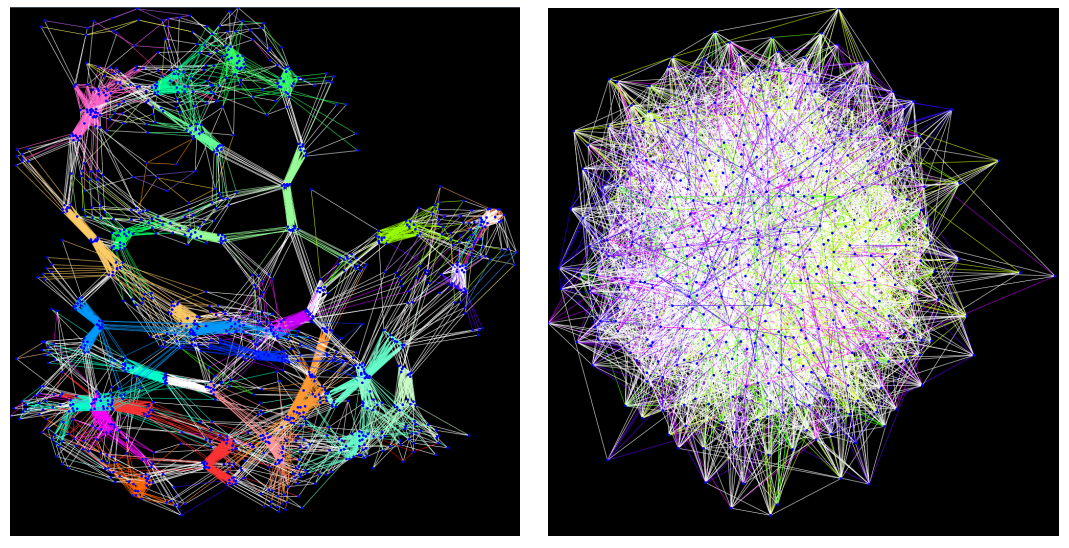
\includegraphics[width=0.7\paperwidth]{chapters/chapter2/sat-graph.png}}
\caption{Сетевая структура индустриальной (слева) и случайно сгенерированной (справа) формул.}
\label{chapter1:fig:satgraph}
\end{figure}

В качестве примера удачной реализации стратегии \enquote{разделяй и властвуй} можно привести проект построения распределенного \textit{SAT}-решателя \textit{SAT@home} [10], выполненного на платформе для GRID-вычислений \textit{BOINC}, реализованный лабораторией Дискретного анализа и прикладной логики Института динамики систем и теории управления СО РАН, позволивший, в числе прочего, найти несколько ортогональных пар диагональных латинских квадратов порядка $10$.

Не все алгоиртмы являются полными в том смысле, что не гарантируют при любом входе завершиться с корректным ответом. Часто отсутствие полноты становится платой за введение дополнитальных эвристик, которые могут значительно ускорить решение задач некоторого класса. 
Многие реализации алгоритма \textit{CDCL} в случае невыполнимости КНФ позволяют построить \enquote{сертификат невыполнимости} в одном из общепринятых форматов (\textit{TraceCheck}, \textit{DRUP} [8]), которое можно верифицировать специальной утилитой, человеку это сделать обычно не под силу. 
Так, группе ученых во главе с Марином Хойле удалось с помощью \textit{SAT}-решателя и суперкомпьютера \textit{Stampede} ($800$ ядер) построить доказательство в формате \textit{DRAT} отсутствия такой двухцветной раскраски множества $\{1, \dots, 7825\}$, при которой ни одна пифагорова тройка из этого множества не является одноцветной (булева проблема пифагоровых троек) [9]. Размер файла с доказательством достиг $200$ терабайт. Такой метод доказательства утверждений используется все чаще, хотя и не приветствуется математическим сообществом.

\begin{figure}[h]
\centering
\captionsetup{justification=centering}
\center{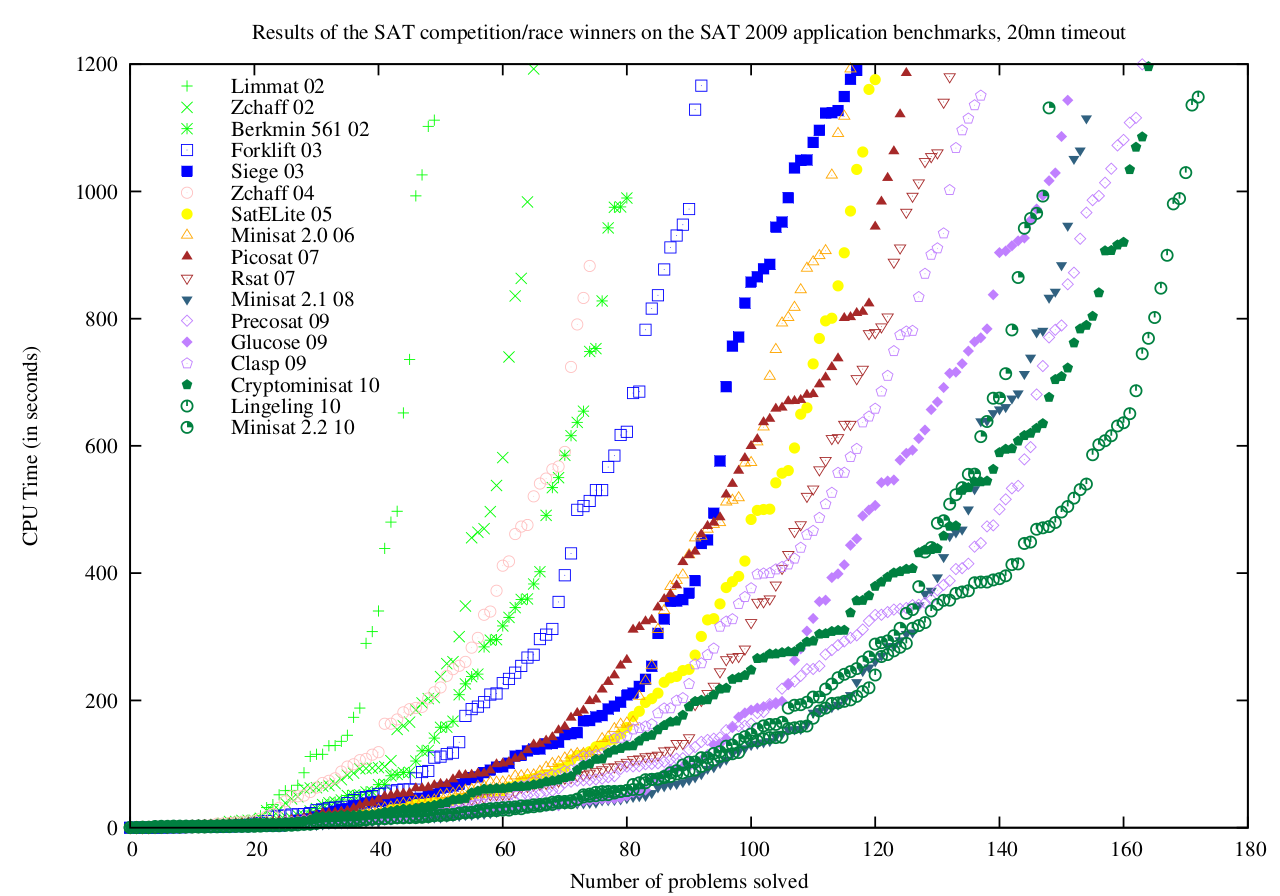
\includegraphics{chapters/chapter2/sat-competition.png}}
\caption{Результаты The International SAT Competition 2009 года.}
\label{chapter1:fig:satcomp}
\end{figure}

На протяжении двух десятков лет проводятся международные состязания по решению задачи \textit{SAT} [11, 12], на которых участники соревнуются в скорости решения специально подобранных задач, записанных в стандартном формате \textit{DIMACS}, при различных условиях (последовательные, параллельные вычисления) и ограничениях. Построение коротких и \enquote{сложных} конкурсных задач, а также формализация свойств формулы, которые делают ее сложной для \enquote{SAT}-решателя – отдельная интересная проблема. Результаты соревнования 
(\figurename{ \ref{chapter1:fig:satcomp}}) публикуются на сайте \url{http://www.satcompetition.org/}. Победителями этого соревнования в разные годы становились \textit{MiniSAT}, \textit{Glucose}, \textit{Lingeling}, \textit{CryptoMiniSat}, \textit{YalSAT}, \textit{MapleSAT}, \textit{abcdSAT}, \textit{RISS}. Все эти проекты имеют открытый исходный код и доступны для свободного использования. Группа ученых из Университета Британской Колумбии поддерживает коллекцию \textit{SAT}-задач различного уровня сложности, известную как бенчмарк \textit{SATLIB} [13]. На протяжении многих лет наилучшие результаты на таких соревнованиях, а также и при решении практических задач, показывают алгоритмы, базирующиеся на идее \textit{CDCL}, о который и пойдет речь далее в этой главе.

\vspace{5pt}
\textbf{2.2. Алгоритм DPLL}\label{chapters:2.2}
\vspace{5pt}

Алгоритма \textit{DPLL} [4] – это полный и высокоэффективный алгоритм решения задачи выполнимости, основанный на классическом алгоритме решения задач комбинаторной оптимизации: поиск в глубину с возвратом. Он назван в честь своих авторов: Дэвиса, Патнема, Логемана, Лавленда, впервые опубликован в 1962 году и является усовершенствованной версией \textit{DP}, предыдущего алгоритма Дэвиса и Патнема, основанного на методу резолюций.

Далее введем несколько общепринятых в литературе обозначений. 
Поскольку порядок элементов не важен, здесь и далее формулу $\Phi$ удобно представлять как множество дизъюнктов $\{ D_1, \dots, D_k \}$, 
каждый из которых является множеством литералов $\{ t_{j,1}, \dots ,t_{j,n_j} \}$ над переменными из множества $X$. Если множество дизъюнктов пусто, формула считается тривиально выполнимой, если один из дизъюнктов пуст - не выполнимой.
В контексте алгоритмов поиска выполняющих наборов каждая переменная $x \in  X$ может находиться в разных состояниях. Переменной может быть присвоено значение $\nu(x)$, $\nu: X \mapsto \{ 0, 1, ?\}$, где знаком \enquote{$?$} обозначается, что значение переменной не определено. Если $\forall x \in X $ $\nu(x) \in \{ 0, 1\}$, то присваивание называется \textit{полным}, иначе - \textit{частичным}. Присваивание $\nu$ позволяет вычислить значения литерала $l^{\nu}$, дизъюнкта $D^{\nu}$ и всей формулы $\Phi^{\nu}$, в этом случае говорят, что им присвоено соответствующее значение. Переменная называется \textit{чистой}, 
если она входит в формулу либо только с отрицанием, либо только без отрицания. \textit{Чистую} переменную (и все ее дизъюнкты) можно удалить из формулы, не нарушив ее выполнимость, такая операция называется \textit{удаление чистых переменных}. 

В ходе вычислений каждый дизъюнкт, в зависимости от функции присваивания, можно охарактеризовать одним из четырех состояний: \textit{невыполненный}, \textit{выполненный}, \textit{единичный}, \textit{неопределенный}. Дизюнкт называется невыполненным, если всем его литералам присвоен $0$, выполненным, если хотя бы одному из его литералов присвоено значение $1$, единичным, если всем литералам, кроме одного, значение которого не определено, присвоено значение $1$, в остальных случаях дизюнкт считается неопределенным. Конечная цель алгоритма - сделать все дизъюнкты выполненными путем присваивания переменным значений.

Ключевой процедурой алгоритма \textit{DPLL} является \textit{разрешение булевых ограничений}. 
Если на каком-то этапе вычислений в формуле появился единичный дизъюнкт, то сделать его выполненным можно только одним способом: выбрать подходящее значение неопределеной переменной, которое называется \textit{предполагаемым}. На этом этапе возможен \textit{конфликт}: 
два разных дизъюнкта могут \enquote{потребовать} одновременно противоположных значений переменной. В ситуации конфликта присваивания, 
которые послужили причиной конфликта (антецедент, $\alpha(x)$), отменяются, алгоритм возвращается на шаг назад. Базовый алгоритм является рекурсивным, поэтому можно ввести понятие \textit{уровня присваивания} переменной $\delta(x)$, который равень уровню рекурсии, на котором было выполнено присваивание. Для неопределенных переменных $\delta(x)=-1$, для предполагаемых $\delta(x)$ равно максимальному из уровней присваиваний антецедентов. На практике разрешение булевых ограничений приводит к каскадному сокращению формулы. 
Обозначения $x = v @ d$, $d/x=v$ эквивалентны $\delta(x) = d$ и $\nu(x) = v$.

Основная схема алгоритма: по некоторому правилу выбрать из множества неопределенных переменных \textit{переменную ветвления}, присвоить ей некоторое значение, сохранить его в \textit{стеке присваиваний}, преобразовать формулу. Затем рекурсивно проверяется выполнимость новой формулы: если она выполнима, то и исходная формула была выполнимой, алгоритм завершает работу с результатом \textit{SAT}, в противном случае (обнаружен конфликт) запустить ту же процедуру, используя противоположное значение переменной. 
Если оба значения выбранной переменной привели к конфликту, алгоритм возвращется на шаг назад, выталкивая одно присваивание из стека. Если возвращаться \enquote{некуда}, алгоритм возвращает \textit{UNSAT}. 
В общем случае алгоритм завершает работу с результатом \textit{UNSAT}, если был выполнен полный перебор всевозможных комбинаций значений переменных.

Преобразование формулы состоит из следующих шагов:
\begin{enumerate}[label=\arabic{*}.]
\item
Из формулы удаляются все дизъюнкты, которые стали выполненными после присваивания переменной, 
все остальные вхождения этой переменной удаляются.
\item Выполняется разрешение булевых ограничений.
\item Выполняется удаление чистых переменных.
\end{enumerate}

Псевдокод алгоритма можно записать следующим образом:

\definecolor{codegreen}{rgb}{0,0.6,0}
\definecolor{codegray}{rgb}{0.5,0.5,0.5}
\definecolor{codepurple}{rgb}{0.58,0,0.82}
\definecolor{backcolour}{rgb}{0.95,0.95,0.92}

\lstdefinestyle{mystyle}{    
    keywordstyle=\color{magenta},
    commentstyle=\color{codegreen},
    lineskip=1ex,
    numberstyle=\tiny\color{codegray},
    stringstyle=\color{codepurple},
    basicstyle=\ttfamily\small,
    breakatwhitespace=false,         
    breaklines=true,                 
    captionpos=b,                    
    keepspaces=true,                 
    numbers=left,                    
    numbersep=5pt,                  
    showspaces=false,                
    showstringspaces=false,
    showtabs=false,                  
    tabsize=2
}

\lstset{style=mystyle}

\lstset{xleftmargin=1.5cm,frame=tlbr,framesep=8pt,framerule=0pt}

\begin{lstlisting}[language=Python, mathescape=true]
def DPLL($\Phi$):	
	$\Phi$ = preprocess($\Phi$)
 	$\Phi$ = pure_literal_elimination($\Phi$)
 	$\Phi$ = unit_propagation($\Phi$)	
	if $\Phi=\{\}$:
		return SAT
	if $\{\} \in \Phi$:
		return UNSAT
 	x = choose_literal($\Phi$)
	return DPLL($\Phi \land \{x\}$) or DPLL($\Phi \land \{\overline{x}\}$)
\end{lstlisting}

\vspace{5pt}

Доработка этого алгоритма ведется в нескольких направлениях:

\begin{enumerate}[label=\arabic{*}.]
\item Построение различных эвристических правил выбора переменной ветвления и соответствующего литерала.
\item Построение ленивых структур данных, позволяющих ускорить отдельные шаги вычисления и сократить объем используемой памяти.
\item Использование \enquote{нехронологических} возвратов и \enquote{запоминание} конфликтных дизъюнктов. 
\end{enumerate}

Последняя идея привела к созданию алгоритма \textit{CDCL}, который является ядром практически всех современных \textit{SAT}-решателей.

\vspace{5pt}
\textbf{2.3. Алгоритм CDCL}\label{chapters:2.3}
\vspace{5pt}

Текст

\vspace{5pt}
\textbf{2.4. Детали реализации современных SAT-решателей}\label{chapters:2.4}
\vspace{5pt}

В этом разделе рассатриваются некоторые технические аспекты реализации \textit{SAT}-решателей, такие как экристики ветвления, случайные рестарты, наблюдаемые литералы, структура данных, методы подбора параметров, которые сыграли ключевую роль [22] в успешности современных алгоритмов. Стоит отметить, что это далеко не исчерпывающий список приемов и их всестороннее исследование может стать темой отдельной работы.

\textbf{Эвристики ветвления}

\textit{Эвристикой ветвления} называется алгоритм выбора переменной ветвления. Простейший способ, в данном случае, - случайный выбор. Еще один возможный вариант - выбирать ту переменную, присваивание которой порождает как можно больше единичных дизъюнктов.
Парадоксально, но случайный выбор нередко позволяет получить результат быстрее прочих, поэтому все эвристики так или иначе включают элемент случайности. 
С другой стороны, в ходе вычислений решатель накапливает определенную информацию, которую можно использовать при выборе переменной ветвления для того, чтобы ускорить вычислительный процесс, сделать его более направленным и контролируемым, а не полагаться на волю случая. 

В литературе предложен ряд эффективных методов, которые используют динамическую информацию о ходе вычислений, структуре конфликтов [18], имеют некоторые теоретические обоснования и широко используются на практике. Ключевая идея: каким-либо образом оценить \enquote{важность} переменной, используя имеющиеся данные. Стоит отметить, что вычисление такой характеристики может быть достаточно \enquote{дорогим}, поэтому нередко умозрительно удачные, но \enquote{тяжелые} подходы проигрывают на практике. Далее рассматривается несколько наиболее популярных методов.

На случайно сгенерированных задачах лучшие результаты показывает эвристика, предложенная \textbf{Bohm}: на каждом шаге из множества неопредленных переменных выбирается переменная с максимальным значением вектора 
$H_i(x_i) = \left(H_1(x_i), \dots, H_m(x_i)\right)$ 
(в смысле лексикографического порядка), где
$H(x) = \alpha \max \{ h_i(x), h_i(\overline{x}) \} + \beta \min \{ h_i(x), h_i(\overline{x}) \}$
и $h_i(x)$ – количество неопределенных дизъюнктов с $i$ литералами, содержащих $x$.
Такая эвристика стремится сделать истинными короткие дизъюнкты (при $x=1$) либо их уменьшить.

Метод \textbf{MOM} (\textit{Maximum Occurrences on Minimum sized clauses}) предлагает выбирать переменную $x$, которая максимизирует функцию 
$S(x) = \left(f^{*}(x) + f^{*}(\overline{x})\right) \cdot 2^{k} + f^{*}(x) \cdot f^{*}(\overline{x})$, где $f^{*}(l)$ - это количество вхождений литерала $l$ в невыполненные дизъюнкты минимального размера. Этот метод выделяет переменные, которые входят в большое количество коротких дизъюнкций с отрицанием или без (при достаточно большом $k$) и одновременно.

Эвристика \textbf{Jeroslow-Wang} устроена следующим образом. Для литерала $l$ вычисляется $J(l) = \sum_{D \in \Phi} 2^{-\left|D\right|}$
Односторонний вариант \textbf{JW-OS} предполагает выбор литерала $l$ с наибольшим значением $J(l)$. Двусторонний \textbf{JW-TS} – поиск переменной $x$ с наибольшей суммой $J(x)+J(\overline{x})$ и присваивание ей $1$, если $J(x) \ge J(\overline{x})$. Такой метод стремится выбирать переменные, которые часто встречаются в коротких дизъюнктах.

\textbf{Эвристики подсчета литералов} устроены значительно проще предыдущих и имеют очевидный интуитивный смысл. Пусть $C_p(x)$ - количество неопределенных дизъюнкций, в которые $x$ входит без отрицания, $C_n(x)$ - с отрицанием. 
Характеристики $C_p(x)$ и $C_n(x)$ можно учитывать в сумме или по отдельности:

\begin{enumerate}[label=\arabic{*}.]
\item Выбрать $x$, для которого $C_p(x) + C_n(x)$ максимальна (\textbf{DLCS}) и присваиванить ей $1$, если $C_p(x) \ge C_n(x)$.
\item Выбрать $x$, для которого $C_p(x)$ ($C_n(x)$) максимальна (\textbf{DLIS}) и присвоить ей заналогично предыдущему пункту (\textbf{DLIS}) или случайно (\textbf{RDLIS}).
\end{enumerate}

Характеристика \textbf{VSIDS} (\textit{Variable State Independent Decaying Sum}) основана на анализе конфликтов и вычисляется инкрементально:

\begin{enumerate}[label=\arabic{*}.]
\item На старте каждым литералом ассоциируется счетчик с нулевым значением.
\item При добавлении очередной \enquote{выученной} дизъюнкции счетчик, ассоциированный с каждым литералом из этой дизъюнкции, увеличивается на $1$.
\item С некоторым периодом все счетчики делятся на константу.
\end{enumerate}

На шаге ветвления выбирается литерал с наибольшим значением счетчика (случайно в случае ничьей). Такая эвристика стремится удовлетворить последние конфликтные дизъюнкты и направляет процесс поиска в сторону их разрешения, что может быть особенно эффективно при решении сложных задач (например, задач с функциональными зависимостями между переменными, в которых конфликты возникают часто). Ее подсчет достаточно прост с вычислительной точки зрения: счетчики обновляются только в случае конфликта.

Метод \textbf{LEFV} (\textit{Last Encountered Free Variable}) очень быстр и хорошо подходит для невыполнимых формул: запоминается неопределенная переменная, которую алгоритм \enquote{встретил} последней на этапе разрешения булевых ограничений. На этапе ветвления выбирается отмеченная переменная, если ее значение все еще не определено, иначе - случайная.


\newpage
\begin{center}
\noindent\textbf{ЗАКЛЮЧЕНИЕ}\label{chapters:conclusions}
\vspace{1.5mm}
\end{center}

В данной работе рассматривалась задача о построении раскрасок двумерных сфер с запрещенными единичными расстояниями. 
В ходе работы были полностью решены все поставленные задачи и получены следующие эмпирические и теоретические результаты:

\begin{enumerate}

\item Установлено, что семейство раскрасок в $8$ и $9$ цветов можно получить на основе сферических диаграмм Вороного, соответствующих локальным минимумам задачи Томсона.  

\item Дан обзор алгоритмов и методов, применяемых при построении современных \textit{SAT}-решателей.

\item Разработан программный код, конструирующий корректные раскраски двумерной сферы на основе решения задачи Томсона.

\item Получены раскраски и оценки хроматических чисел сфер некоторых для диапазонов радиусов.

\item Получены оценки хроматических чисел двойственных графов для регулярных решений задачи Томсона.

\item Разработана программа для визуализации сферических диаграмм Вороного и их раскрасок.

\end{enumerate}

Программный код и все материалы, необходимые для воспроизведения полученных результатов, размещены в открытом доступе по адресу
\url{https://github.com/xm-repo/sphere}.
Несмотря на то, что данная работа является еще одним небольшим шагом к решению задачи о раскраске сфер, полученные результаты нельзя назвать исчерпывающими. Среди открытых вопросов и направлений для дальнейших исследований можно отметить следующие:

\begin{enumerate}

\item Доказательство оценки для хроматического числа квадрата двойственного графа регулярных триангуляций сферы.
\item Доказательство общей оценки хроматического числа сферы для достаточно больших значений радиуса.
\item Постановка и решение аналогичных задач для трехмерных сфер.
\item Изучение случая сферы с радиусом $\frac{1}{2}+\varepsilon$.

\end{enumerate}



\newpage
\begin{center}
\noindent\textbf{СПИСОК ИСПОЛЬЗОВАННЫХ ИСТОЧНИКОВ}\label{chapters:biblio}
\vspace{1.5mm}
\end{center}

\begin{enumerate}[leftmargin=0.5cm,topsep=0pt,itemsep=-1ex,partopsep=1ex,parsep=1ex,label=\arabic{*}.]

\item
Cook S. A. The complexity of theorem-proving procedures //Proceedings of the third annual ACM symposium on Theory of computing. – 1971. – С. 151-158.

\item
Karp R. M. Reducibility among combinatorial problems //Complexity of computer computations. – Springer, Boston, MA, 1972. – С. 85-103.

\item
Rolf D. Improved bound for the PPSZ/Schöning-algorithm for 3-SAT //Jour\-nal on Satisfiability, Boolean Modeling and Computation. – 2006. – Т. 1. – №. 2. – С. 111-122.

\item
Robinson J. A. Martin Davis, George Logemann, and Donald Loveland. A machine program for theorem-proving. Communications of the ACM, vol. 5 (1962), pp. 394–397 //The Journal of Symbolic Logic. – 1967. – Т. 32. – №. 1. – С. 118-118.

\item
Marques-Silva J., Malik S. Propositional SAT solving //Handbook of Model Checking. – Springer, Cham, 2018. – С. 247-275.

\item
Lardeux F., Saubion F., Hao J. K. GASAT: a genetic local search algorithm for the satisfiability problem //Evolutionary Computation. – 2006. – Т. 14. – №. 2. – С. 223-253.

\item
Selsam D. et al. Learning a SAT solver from single-bit supervision //arXiv preprint arXiv:1802.03685. – 2018.

\item
Heule M., Biere A. Proofs for satisfiability problems //All about Proofs, Proofs for all. – 2015. – Т. 55. – №. 1. – С. 1-22.

\item
Heule M. J. H., Kullmann O., Marek V. W. Solving and verifying the boolean pythagorean triples problem via cube-and-conquer //International Conference on Theory and Applications of Satisfiability Testing. – Springer, Cham, 2016. – С. 228-245.

\item
Zaikin O., Kochemazov S., Semenov A. SAT-based search for systems of diagonal latin squares in volunteer computing project sat@ home //2016 39th International Convention on Information and Communication Technology, Electronics and Microelectronics (MIPRO). – IEEE, 2016. – С. 277-281.

\item
Järvisalo M. et al. The international SAT solver competitions //Ai Magazine. – 2012. – Т. 33. – №. 1. – С. 89-92.
	
\item
Biere A. Cadical, Lingeling, Plingeling, Treengeling and YalSAT entering the sat competition 2018 //Proc. of SAT Competition. – 2018. – С. 13-14.

\item
Hoos H. H., Stützle T. SATLIB: An online resource for research on SAT //Sat. – 2000. – Т. 2000. – С. 283-292.

\item
Hoos H. H., Stützle T. Local search algorithms for SAT: An empirical evaluation //Journal of Automated Reasoning. – 2000. – Т. 24. – №. 4. – С. 421-481.

\item
Sorensson N., Een N. Minisat v1. 13-a sat solver with conflict-clause minimization //SAT. – 2005. – Т. 2005. – №. 53. – С. 1-2.

\item
Biere A., Heule M., van Maaren H. (ed.). Handbook of satisfiability. – IOS press, 2009. – Т. 185.

\item
Puri R., Gu J. A BDD SAT solver for satisfiability testing: An industrial case study //Annals of Mathematics and Artificial Intelligence. – 1996. – Т. 17. – №. 2. – С. 315-337.

\item
Marques-Silva J. The impact of branching heuristics in propositional satisfiability algorithms //Portuguese Conference on Artificial Intelligence. – Springer, Berlin, Heidelberg, 1999. – С. 62-74.

\item
Eén N., Biere A. Effective preprocessing in SAT through variable and clause elimination //International conference on theory and applications of satisfiability testing. – Springer, Berlin, Heidelberg, 2005. – С. 61-75.

\item
Moskewicz M. W. et al. Chaff: Engineering an efficient SAT solver //Proceedings of the 38th annual Design Automation Conference. – 2001. – С. 530-535.

\item
Kullmann O. Theory and applications of satisfiability testing //SAT. – 2009. – С. 147.

\item
Katebi H., Sakallah K. A., Marques-Silva J. P. Empirical study of the anatomy of modern sat solvers //International Conference on Theory and Applications of Satisfiability Testing. – Springer, Berlin, Heidelberg, 2011. – С. 343-356.

\item
Nadel A. Backtrack search algorithms for propositional logic satisfiability: Review and innovations. – Hebrew University of Jerusalem, 2002.


\item
Newsham Z. et al. SATGraf: Visualizing the evolution of SAT formula structure in solvers //International Conference on Theory and Applications of Satisfiability Testing. – Springer, Cham, 2015. – С. 62-70.

\item
Heule M. J. H. Computing small unit-distance graphs with chromatic number 5 //arXiv preprint arXiv:1805.12181. – 2018.

\item
Soifer A. The mathematical coloring book: Mathematics of coloring and the colorful life of its creators. – Springer Science \& Business Media, 2008.

\end{enumerate}


\definecolor{codegreen}{rgb}{0,0.6,0}
\definecolor{codegray}{rgb}{0.5,0.5,0.5}
\definecolor{codepurple}{rgb}{0.58,0,0.82}
\definecolor{backcolour}{rgb}{0.95,0.95,0.92}

\lstdefinestyle{mystyle}{    
    keywordstyle=\color{magenta},
    commentstyle=\color{codegreen},
    lineskip=-1ex,
    numberstyle=\tiny\color{codegray},
    stringstyle=\color{codepurple},
    basicstyle=\ttfamily\footnotesize,
    breakatwhitespace=false,         
    breaklines=true,                 
    captionpos=b,                    
    keepspaces=true,                 
    numbers=left,                    
    numbersep=5pt,                  
    showspaces=false,                
    showstringspaces=false,
    showtabs=false,                  
    tabsize=2,
    xleftmargin=0cm
}

\lstset{style=mystyle}


\newpage
\begin{center}
\noindent\textbf{ПРИЛОЖЕНИЕ 1. ДИАПАЗОНЫ ЗНАЧЕНИЙ РАДИУСА ДЛЯ РЕШЕНИЙ ЗАДАЧИ ТОМСОНА}\label{attachments:1}
\vspace{1.5mm}
\end{center}

\begin{longtable}{ccll} 
\hline
n & k & $r_{min}$ & $r_{max}$ \\ 
\hline
\endhead
\input{chapters/attachments/colorings2.txt}
\hline
\end{longtable}

\newpage
\begin{center}
\noindent\textbf{ПРИЛОЖЕНИЕ 2. КОДИРОВАНИЕ ЗАДАЧИ РАСКРАСКИ ГРАФА}\label{attachments:2}
\vspace{1.5mm}
\end{center}

\lstinputlisting[language=Python]{chapters/attachments/g2cnf.py}

\newpage
\begin{center}
\noindent\textbf{ПРИЛОЖЕНИЕ 3. ВЫЧИСЛЕНИЕ ГРАНИЦ ДИАПАЗОНОВ ЗНАЧЕНИЙ РАДИУСА}\label{attachments:3}
\vspace{1.5mm}
\end{center}

\lstinputlisting[language=Python]{chapters/attachments/build_gs.py}

\newpage
\begin{center}
\noindent\textbf{ПРИЛОЖЕНИЕ 4. ПОСТРОЕНИЕ ДИАГРАММЫ ВОРОНОГО С ИКОСАЭДРАЛЬНОЙ СИММЕТРИЕЙ}\label{attachments:4}
\vspace{1.5mm}
\end{center}

\lstinputlisting[language=Python]{chapters/attachments/sphere_triang.py}

\newpage
\begin{center}
\noindent\textbf{ПРИЛОЖЕНИЕ 5. ВИЗУАЛИЗАЦИЯ РАСКРАСОК}\label{attachments:5}
\vspace{1.5mm}
\end{center}

\lstinputlisting[language=C++]{chapters/attachments/Utils.hpp}

\lstinputlisting[language=C++]{chapters/attachments/sphere.cpp}


\end{document}